\chapter{Sizing and Scheduling}
\label{ch:sizeschedule}

\section{Scheduling}
In this section a proposal of scheduling is provided. First of all,, it is necessary to define the extension of the route from the Business Park to Stradella FS, as shown in Figure \ref{fig:path}.

\begin{figure}[h]
    \centering
    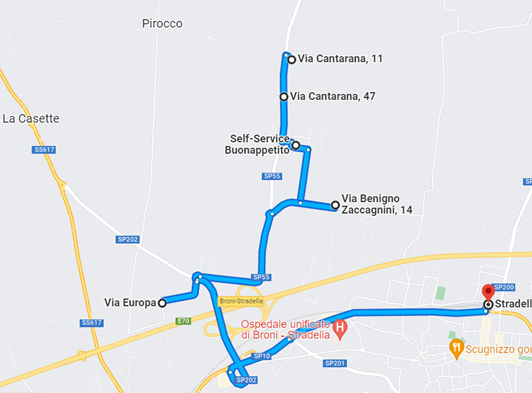
\includegraphics[width=0.7\textwidth]{Images/Scheduling/Path.png}
    \caption{Path from Business Park to Stradella FS}
    \label{fig:path}
\end{figure}




The additional stops, close to access point of the Business Park, will be:
\begin{itemize}
    \item Via Cantarana, 11 San Cipriniano Po
    \item Via Cantarana, 47 San Cipriniano Po
    \item Via dell'Industria, 1, 27049 Stradella PV
    \item Via Benigno Zaccagnini, 14 Stradella
    \item Via Europa, Broni
\end{itemize}


In the following pages the changes to the schedule time are reported. In figure \ref{fig:A1} and \ref{fig:A2} the changes due to the Scenario A (a creation of a tailor-made ride). In figure \ref{fig:B1} and \ref{fig:B2} the changes for scenario B (the modification of an existing ride).

The changes in yellow are consequences of the changes of the last stop of the bus. This has an effect also on the following rides because the bus is not in the same stop of the departure.

For the enter and exit at 6:00 and 22:00 we have only one scenario that consists in the creation of a new ride.

Regarding the changes for the entry at 08:30 in Figure \ref{fig:enter830} we can see the only changes the require the extension of ride 140021. For the exit at 17:30 the timetable is reported in Figure \ref{fig:exit1730}. This change does not impact on the other lines due to a greater headway. In the following section of this chapter a preliminary sizing of the new service is performed, quantifying the additional number of kilometers travelled, working hours and resources.

\newpage
\thispagestyle{empty}
\begin{landscape}
\begin{figure}[h]
    \centering
    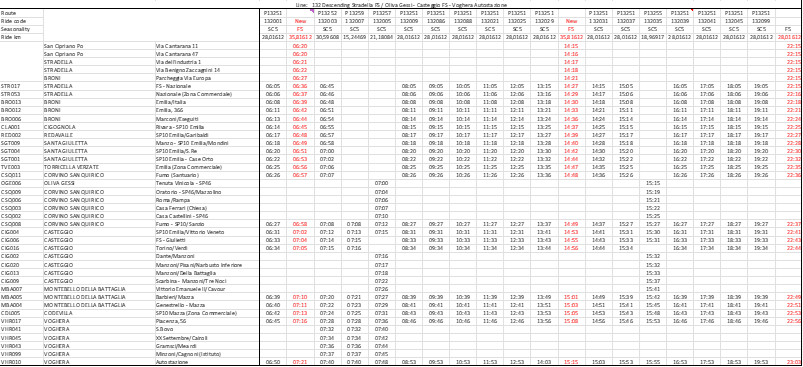
\includegraphics[width=1.4\textwidth]{Images/Scheduling/timetables/Scenario_A.png}
    \caption{Scenario A: Timetables for Enter at 6,14 and 22}
    \label{fig:A1}
\end{figure}
\end{landscape}


\newpage
\thispagestyle{empty}
\begin{landscape}
\begin{figure}[h]
    \centering
    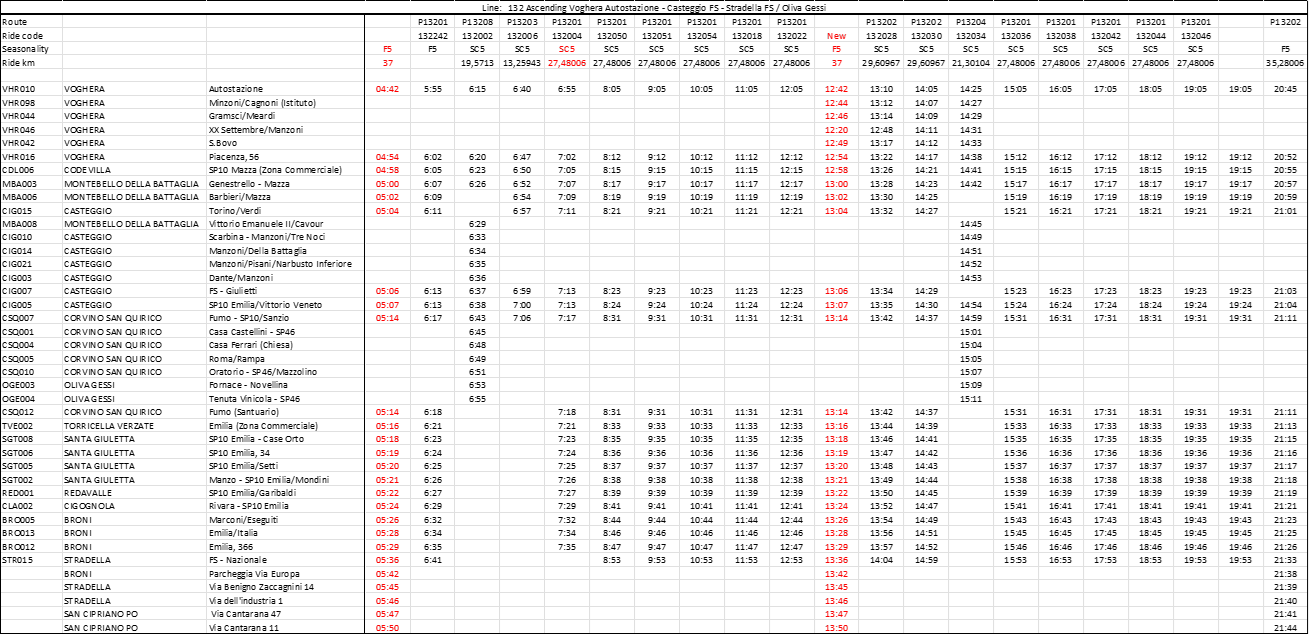
\includegraphics[width=1.4\textwidth]{Images/Scheduling/timetables/Scenario_A_2.png}
    \caption{Scenario A: Timetables for Exit at 6,14 and 22}
    \label{fig:A2}
\end{figure}
\end{landscape}
\newpage
\thispagestyle{empty}
\begin{landscape}
\begin{figure}[h]
    \centering
    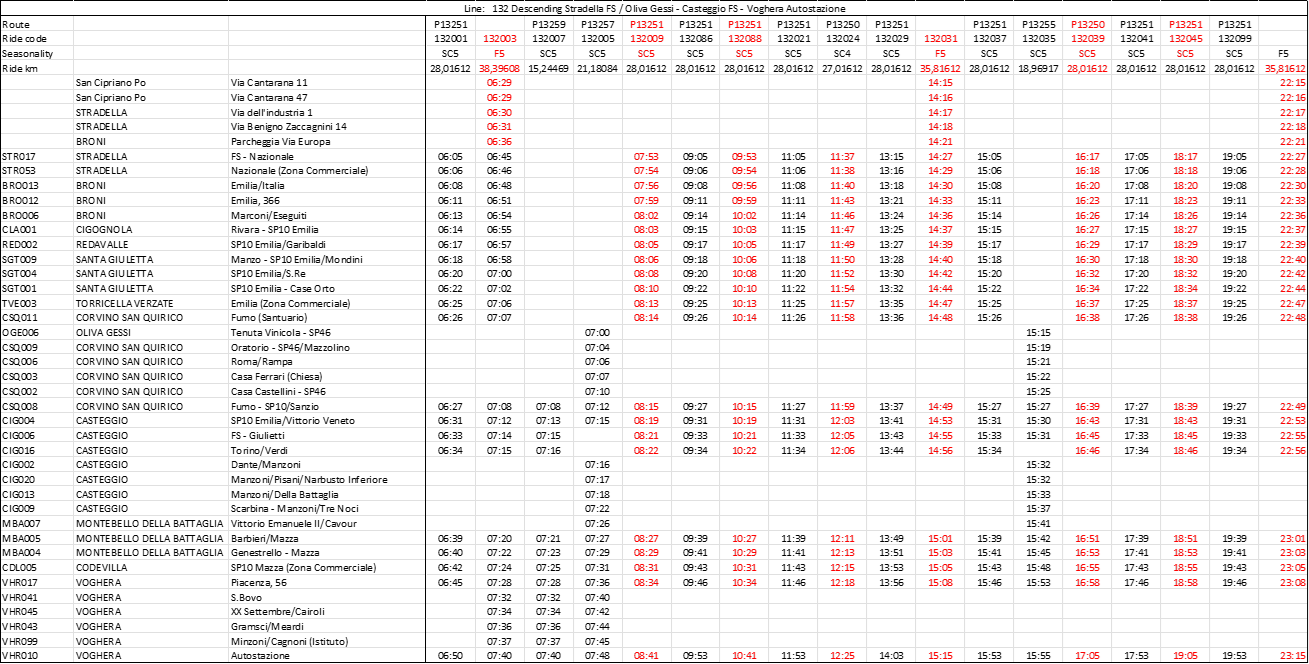
\includegraphics[width=1.4\textwidth]{Images/Scheduling/timetables/Scenario_B.png}
    \caption{Scenario B: Timetables for enter at 6,14 and 22}
    \label{fig:B1}
\end{figure}
\end{landscape}
\newpage
\thispagestyle{empty}
\begin{landscape}
\begin{figure}[h]
    \centering
    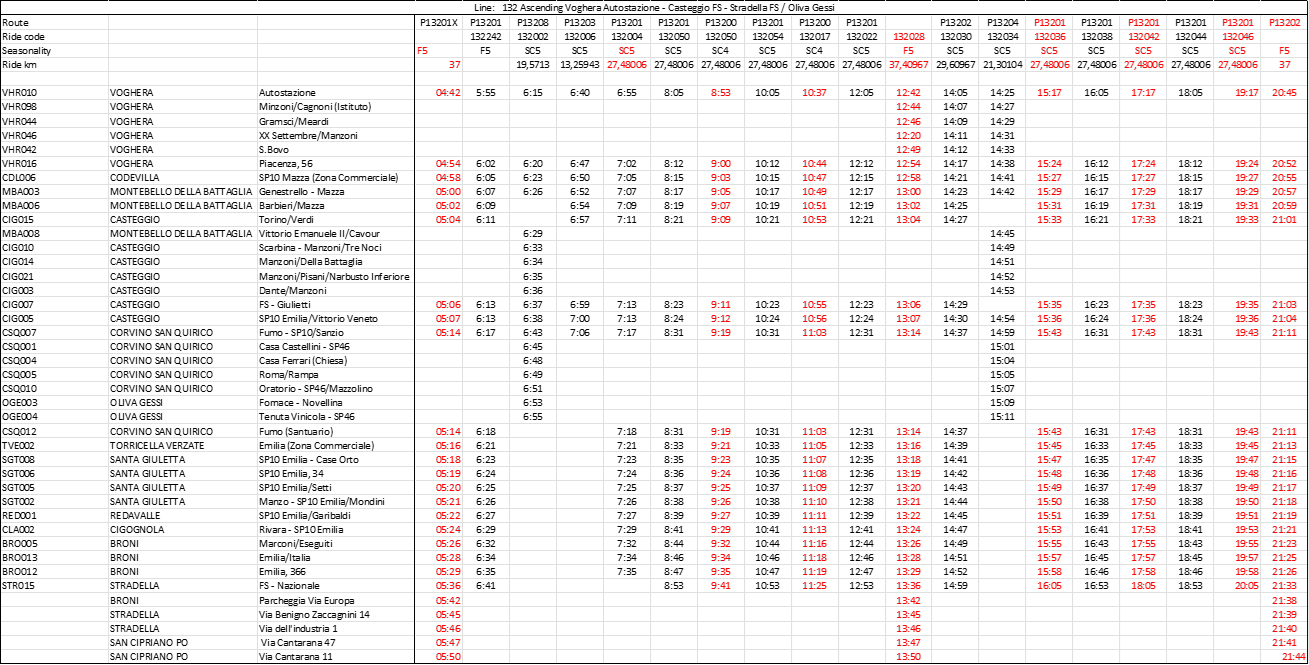
\includegraphics[width=1.4\textwidth]{Images/Scheduling/timetables/Scenario_B_2.png}
    \caption{Scenario B: Timetables for exit at 6,14 and 22}
    \label{fig:B2}
\end{figure}
\end{landscape}
\newpage
\thispagestyle{empty}
\begin{figure}[h]
    \centering
    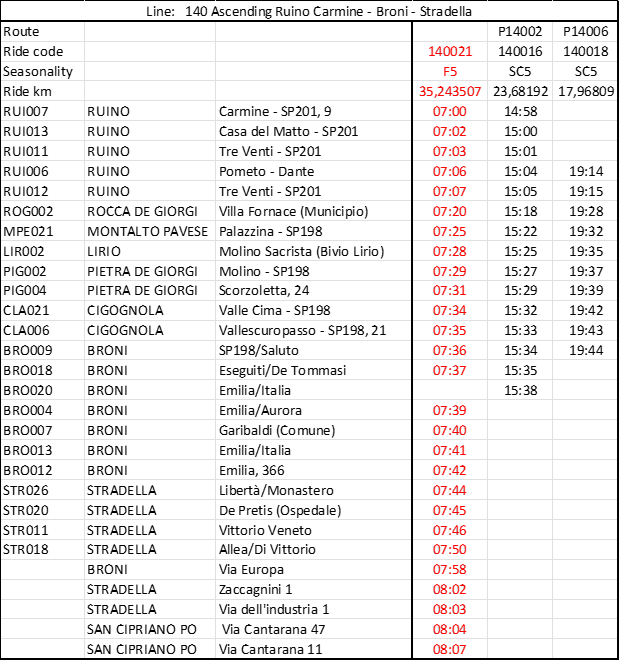
\includegraphics[width=1\textwidth]{Images/Scheduling/timetables/enter_8_30.png}
    \caption{Timetables for enter at 8:30}
    \label{fig:enter830}
\end{figure}
\newpage
\thispagestyle{empty}
\begin{figure}[h!]
    \centering
    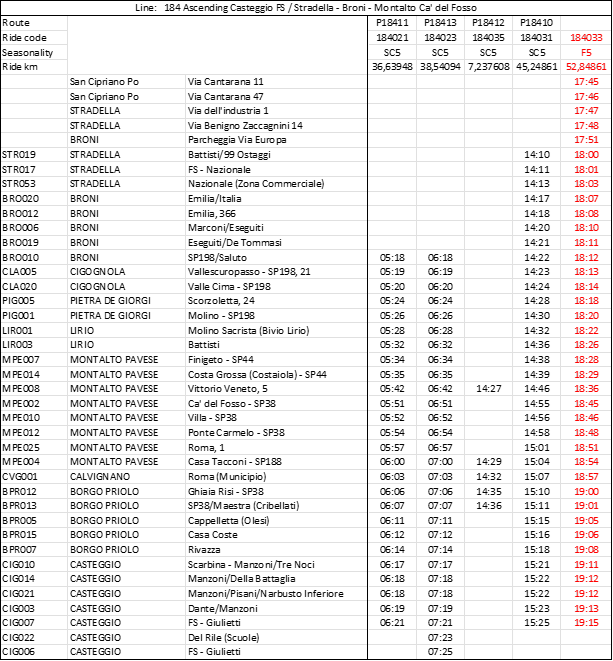
\includegraphics[width=1\textwidth]{Images/Scheduling/timetables/Exit_17_30.png}
    \caption{Timetables for enter at 17:30}
    \label{fig:exit1730}
\end{figure}
\newpage
\newpage

\section{Sizing}
This evaluation will be dependent on the different actions required to fit the new scheduling. In this case two options are available: the creation of a new ride from scratch or, if minor changes are suitable, a slight advance or delay of an existing one. Since the information of drivers and bus shift is not sufficiently detailed so as to integrate changes with the existing one, the assumption was that each new ride requires a dedicated driver and bus.
In detail, the rides requiring an additional bus and drivers are 
\paragraph{Start of shift 6:00}

The solution adopted for this shift is common for both the scenarios: the introduction of an additional ride. This requires an additional bus and driver for 37 km and 68 minutes.
\paragraph{End of shift 6:00}

According to the scheduling, the new ride is performed exploiting the presence of bus and driver in the Business Park for the start of shift 6:00. 
\begin{description}
    \item[Scenario A]: a tailor-made ride is created, with all the consequences implied in terms of kilometers and resources.
    \item[Scenario B]: the modification of an existing ride, extending its path and advancing the schedule.
\end{description}

\paragraph{Start of shift 8:30}

The solution adopted for this shift is common for both the scenarios: the modification of an existing ride extending its path till the Business Park for 4.9 km and 17 minutes, without the need of a new bus and driver.
\paragraph{Start and end of shift 14:00}

The resulting scenarios, for both arrival and departure, follow the same logic presented for the end of shift 6:00. Scenario A consists in the implementation of a completely new ride, while Scenario B exploits existing rides modified in their paths and routes in order to serve the Business Park.

\paragraph{End of shift 17:30}

The solution adopted for this shift is common for both the scenarios: the modification of an existing ride extending its path from the Business Park for 7.6 km and 15 minutes, without the need of a new bus and driver.
\paragraph{Start and end of shift 22:00}

The solutions adopted for both arrival and departure are the implementation of two new rides. Anyway, these two rides share the same bus and driver.

% Please add the following required packages to your document preamble:
% \usepackage{multirow}
% \usepackage[table,xcdraw]{xcolor}
% If you use beamer only pass "xcolor=table" option, i.e. \documentclass[xcolor=table]{beamer}
\begin{table}[h]
\centering
\begin{tabular}{|ll|l|c|c|l|l|l|}
\hline
\rowcolor{bluepoli!40}
\multicolumn{1}{|c|}{\textbf{Shift}} & \multicolumn{1}{c|}{\textbf{\begin{tabular}[c]{@{}c@{}}To/From \\ BP\end{tabular}}} & \multicolumn{1}{c|}{\textbf{km}} & \textbf{Drivers}         & \textbf{Buses}           & \multicolumn{1}{c|}{\textbf{\begin{tabular}[c]{@{}c@{}}time \\ {[}min{]}\end{tabular}}} & \multicolumn{1}{c|}{\textbf{km/year}} & \multicolumn{1}{c|}{\textbf{h/year}} \\ \hline
\multicolumn{1}{|l|}{06:00}          & To                                                                                  & 37                               &                          &                          & 68                                                                                      & 9398                                  & 269                                  \\ \cline{1-3} \cline{6-8} 
\multicolumn{1}{|l|}{06:00}          & From                                                                                & 36                               & \multirow{-2}{*}{1}      & \multirow{-2}{*}{1}      & 61                                                                                      & 9144                                  & 261                                  \\ \hline
\multicolumn{1}{|l|}{08:30}          & To                                                                                  & 4,9                              & 0                        & 0                        & 17                                                                                      & 3409,2                                & 97                                   \\ \hline
\multicolumn{1}{|l|}{14:00}          & To                                                                                  & 37                               &                          &                          & 68                                                                                      & 9398                                  & 269                                  \\ \cline{1-3} \cline{6-8} 
\multicolumn{1}{|l|}{14:00}          & From                                                                                & 36                               & \multirow{-2}{*}{1}      & \multirow{-2}{*}{1}      & 60                                                                                      & 9144                                  & 261                                  \\ \hline
\multicolumn{1}{|l|}{17:30}          & From                                                                                & 7,6                              & 0                        & 0                        & 15                                                                                      & 5485,4                                & 157                                  \\ \hline
\multicolumn{1}{|l|}{22:00}          & To                                                                                  & 35                               &                          &                          & 55                                                                                      & 8890                                  & 254                                  \\ \cline{1-3} \cline{6-8} 
\multicolumn{1}{|l|}{22:00}          & From                                                                                & 36                               & \multirow{-2}{*}{1}      & \multirow{-2}{*}{1}      & 60                                                                                      & 9144                                  & 261                                  \\ \hline
\multicolumn{2}{|l|}{sum}                                                                                                  & 229.5                            & 3 & 3 & 404                                                                                     & 64012,6                               & 1829                                 \\ \hline
\end{tabular}
\caption{Scenario A: additional resources}
\label{tab:addresA}
\end{table}

% Please add the following required packages to your document preamble:
% \usepackage{multirow}
\begin{table}[h]
\centering
\begin{tabular}{|ll|l|l|l|l|l|l|}
\hline
\rowcolor{bluepoli!40}
\multicolumn{1}{|c|}{\textbf{Shift}} & \multicolumn{1}{c|}{\textbf{\begin{tabular}[c]{@{}c@{}}To/From \\ BP\end{tabular}}} & \multicolumn{1}{c|}{\textbf{Km}} & \multicolumn{1}{c|}{\textbf{Drivers}} & \multicolumn{1}{c|}{\textbf{Buses}} & \multicolumn{1}{c|}{\textbf{\begin{tabular}[c]{@{}c@{}}time \\ {[}min{]}\end{tabular}}} & \multicolumn{1}{c|}{\textbf{km/year}} & \multicolumn{1}{c|}{\textbf{h/year}} \\ \hline
\multicolumn{1}{|l|}{06:00}          & To                  & 37          & 1                  & 1                  & 68                      & 9398             & 269                 \\ \hline
\multicolumn{1}{|l|}{06:00}          & From                & 7.8         & 0                  & 0                  & 16                      & 3614,6           & 103                 \\ \hline
\multicolumn{1}{|l|}{08:30}          & To                  & 4.9         & 0                  & 0                  & 17                      & 3409,2           & 97                  \\ \hline
\multicolumn{1}{|l|}{14:00}          & To                  & 7.8         & 0                  & 0                  & 14                      & 11514            & 329                 \\ \hline
\multicolumn{1}{|l|}{14:00}          & From                & 7.8         & 0                  & 0                  & 12                      & 4300,4           & 123                 \\ \hline
\multicolumn{1}{|l|}{17:30}          & From                & 7.6         & 0                  & 0                  & 15                      & 11260            & 322                 \\ \hline
\multicolumn{1}{|l|}{22:00}          & To                  & 35          & \multirow{2}{*}{1} & \multirow{2}{*}{1} & 55                      & 8890             & 254                 \\ \cline{1-3} \cline{6-8} 
\multicolumn{1}{|l|}{22:00}          & From                & 36          &                    &                    & 60                      & 9144             & 261                 \\ \hline
\multicolumn{2}{|l|}{sum}                                  & 143.9       & 2                  & 2                  & 257                     & 61530,2          & 1758                \\ \hline
\end{tabular}
\caption{Scenario B: Additional resource}
\label{tab:addresB}
\end{table}

With the scenario B (changes of the rides) solution about 2500 km/year and 71 hours/year are saved.

Some remarks on table \ref{tab:addresA} and \ref{tab:addresB}:
\begin{enumerate}
    \item Since the working hours of a driver is generally 6 hours, probably it should be enough for Scenario A to add only two drivers ($404 min/(60 min/h \cdot 6 h/driver) = 1.12 drivers \approx 2 drivers$), while for Scenario B one driver is enough.
    \item Since the rides are not at the same time, probably only one bus should be enough for both the Scenarios
\end{enumerate}